\documentclass[leqno, 12pt]{article}
\usepackage{tikz}
\usepackage{amsmath}
\usepackage{ulem}
\usetikzlibrary{angles,quotes,intersections,arrows.meta,calc}
\usepackage[a4paper, portrait, margin=1cm]{geometry}
\usepackage{multicol}
\usepackage{fancyhdr}

\def \HeadingQuestions {\section*{\Large Name: \underline{\hspace{8cm}} \hfill Date: \underline{\hspace{3cm}}} \vspace{-3mm}
{Parallel lines Angles: Questions} \vspace{1pt}\hrule}

% raise footer with page number; no header
\fancypagestyle{myfancypagestyle}{
  \fancyhf{}% clear all header and footer fields
  \renewcommand{\headrulewidth}{0pt} % no rule under header
  \fancyfoot[C] {\thepage} \setlength{\footskip}{14.5pt} % raise page number allowed min 14.5pt
}
\pagestyle{myfancypagestyle}  % apply myfancypagestyle


\begin{document}
\HeadingQuestions
\begin{multicols}{2}


\begin{equation}
  \text{e} = \text{\dotuline{~~~~~~~}}^\circ
  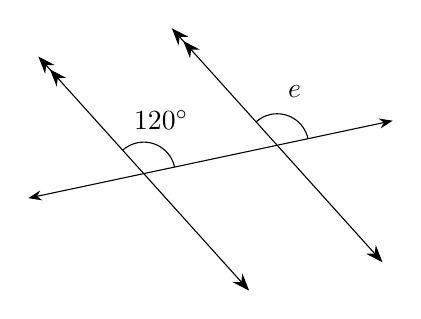
\begin{tikzpicture}[scale=1.0, baseline=(current bounding box.north)]
    \begin{scope}[rotate=12]
      % Draw the first line
      \draw[<->>, >={Stealth[scale=1.3]}, name path=P1] (0, 0) -- (-1.9999999999999991, 3.464101615137755);
      % Draw the second line with the calculated offsets
      \draw[<->>, >={Stealth[scale=1.3]}, name path=P2] (1.7320508075688772, 0) -- (-0.2679491924311219, 3.464101615137755);
      % Draw the transversal through the middle of the parallel lines
      \draw[<->, >=Stealth, name path=P3] (-2.499999999999999, 1.7320508075688774) -- (2.2320508075688776, 1.7320508075688774);
      \path [name intersections={of=P1 and P3,by=A}];
      \path [name intersections={of=P2 and P3,by=B}];
      % Draw the angle
      \coordinate (p1s) at (0, 0);
      \coordinate (p1e) at (-1.9999999999999991, 3.464101615137755);
      \coordinate (p2s) at (1.7320508075688772, 0);
      \coordinate (p2e) at (-0.2679491924311219, 3.464101615137755);
      \coordinate (ts) at (-2.499999999999999, 1.7320508075688774);
      \coordinate (te) at (2.2320508075688776, 1.7320508075688774);
      \draw pic["$e$", draw=black, -, angle eccentricity=1.8, angle radius=0.4cm] {angle=te--B--p2e};
\draw pic["$120^\circ$", draw=black, -, angle eccentricity=1.8, angle radius=0.4cm] {angle=te--A--p1e};

    \end{scope}
  \end{tikzpicture}
\end{equation}\vspace{1cm}
\begin{equation}
  \text{g} = \text{\dotuline{~~~~~~~}}^\circ
  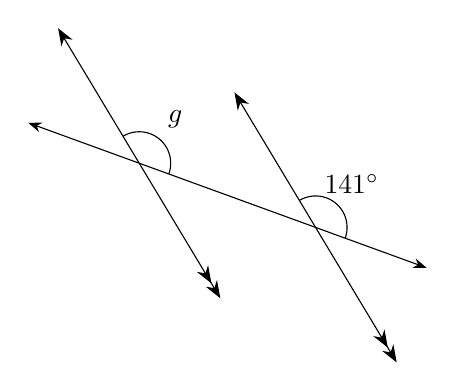
\begin{tikzpicture}[scale=1.0, baseline=(current bounding box.north)]
    \begin{scope}[rotate=160]
      % Draw the first line
      \draw[<->>, >={Stealth[scale=1.3]}, name path=P1] (0, 0) -- (-3.1085838458278836, 2.5172815641993496);
      % Draw the second line with the calculated offsets
      \draw[<->>, >={Stealth[scale=1.3]}, name path=P2] (2.3835235935986243, 0) -- (-0.7250602522292593, 2.5172815641993496);
      % Draw the transversal through the middle of the parallel lines
      \draw[<->, >=Stealth, name path=P3] (-3.054291922913942, 1.2586407820996748) -- (2.329231670684682, 1.2586407820996748);
      \path [name intersections={of=P1 and P3,by=A}];
      \path [name intersections={of=P2 and P3,by=B}];
      % Draw the angle
      \coordinate (p1s) at (0, 0);
      \coordinate (p1e) at (-3.1085838458278836, 2.5172815641993496);
      \coordinate (p2s) at (2.3835235935986243, 0);
      \coordinate (p2e) at (-0.7250602522292593, 2.5172815641993496);
      \coordinate (ts) at (-3.054291922913942, 1.2586407820996748);
      \coordinate (te) at (2.329231670684682, 1.2586407820996748);
      \draw pic["$g$", draw=black, -, angle eccentricity=1.8, angle radius=0.4cm] {angle=ts--B--p2s};
\draw pic["$141^\circ$", draw=black, -, angle eccentricity=1.8, angle radius=0.4cm] {angle=ts--A--p1s};

    \end{scope}
  \end{tikzpicture}
\end{equation}\vspace{1cm}
\begin{equation}
  \text{h} = \text{\dotuline{~~~~~~~}}^\circ
  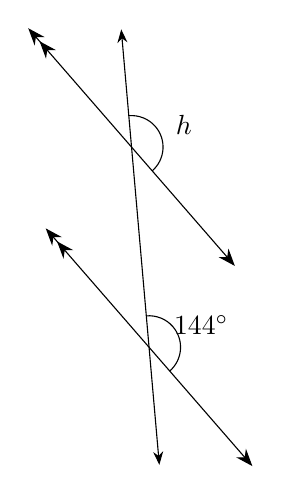
\begin{tikzpicture}[scale=1.0, baseline=(current bounding box.north)]
    \begin{scope}[rotate=95]
      % Draw the first line
      \draw[<->>, >={Stealth[scale=1.3]}, name path=P1] (0, 0) -- (3.23606797749979, 2.3511410091698925);
      % Draw the second line with the calculated offsets
      \draw[<->>, >={Stealth[scale=1.3]}, name path=P2] (2.5519524250561196, 0) -- (5.78802040255591, 2.3511410091698925);
      % Draw the transversal through the middle of the parallel lines
      \draw[<->, >=Stealth, name path=P3] (0.1180339887498949, 1.1755705045849463) -- (5.669986413806015, 1.1755705045849463);
      \path [name intersections={of=P1 and P3,by=A}];
      \path [name intersections={of=P2 and P3,by=B}];
      % Draw the angle
      \coordinate (p1s) at (0, 0);
      \coordinate (p1e) at (3.23606797749979, 2.3511410091698925);
      \coordinate (p2s) at (2.5519524250561196, 0);
      \coordinate (p2e) at (5.78802040255591, 2.3511410091698925);
      \coordinate (ts) at (0.1180339887498949, 1.1755705045849463);
      \coordinate (te) at (5.669986413806015, 1.1755705045849463);
      \draw pic["$h$", draw=black, -, angle eccentricity=1.8, angle radius=0.4cm] {angle=p2s--B--te};
\draw pic["$144^\circ$", draw=black, -, angle eccentricity=1.8, angle radius=0.4cm] {angle=p1s--A--te};

    \end{scope}
  \end{tikzpicture}
\end{equation}\vspace{1cm}
\begin{equation}
  \text{e} = \text{\dotuline{~~~~~~~}}^\circ
  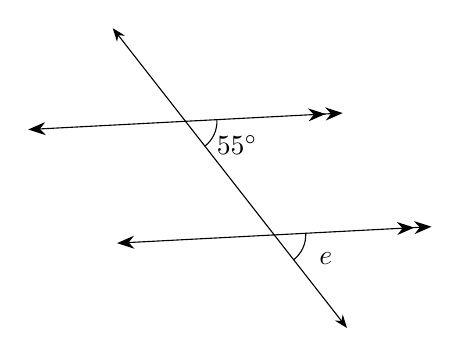
\begin{tikzpicture}[scale=1.0, baseline=(current bounding box.north)]
    \begin{scope}[rotate=308]
      % Draw the first line
      \draw[<->>, >={Stealth[scale=1.3]}, name path=P1] (0, 0) -- (2.294305745404184, 3.276608177155967);
      % Draw the second line with the calculated offsets
      \draw[<->>, >={Stealth[scale=1.3]}, name path=P2] (1.831161883142184, 0) -- (4.125467628546368, 3.276608177155967);
      % Draw the transversal through the middle of the parallel lines
      \draw[<->, >=Stealth, name path=P3] (-0.3528471272979079, 1.6383040885779836) -- (4.478314755844276, 1.6383040885779836);
      \path [name intersections={of=P1 and P3,by=A}];
      \path [name intersections={of=P2 and P3,by=B}];
      % Draw the angle
      \coordinate (p1s) at (0, 0);
      \coordinate (p1e) at (2.294305745404184, 3.276608177155967);
      \coordinate (p2s) at (1.831161883142184, 0);
      \coordinate (p2e) at (4.125467628546368, 3.276608177155967);
      \coordinate (ts) at (-0.3528471272979079, 1.6383040885779836);
      \coordinate (te) at (4.478314755844276, 1.6383040885779836);
      \draw pic["$e$", draw=black, -, angle eccentricity=1.8, angle radius=0.4cm] {angle=te--B--p2e};
\draw pic["$55^\circ$", draw=black, -, angle eccentricity=1.8, angle radius=0.4cm] {angle=te--A--p1e};

    \end{scope}
  \end{tikzpicture}
\end{equation}\vspace{1cm}
\begin{equation}
  \text{e} = \text{\dotuline{~~~~~~~}}^\circ
  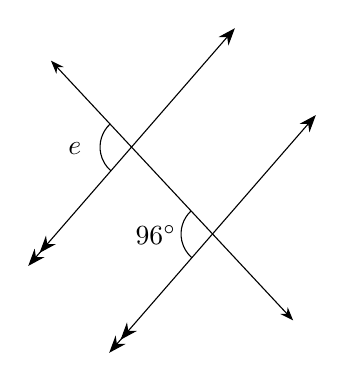
\begin{tikzpicture}[scale=1.0, baseline=(current bounding box.north)]
    \begin{scope}[rotate=133]
      % Draw the first line
      \draw[<->>, >={Stealth[scale=1.3]}, name path=P1] (0, 0) -- (-0.4181138530706142, 3.978087581473093);
      % Draw the second line with the calculated offsets
      \draw[<->>, >={Stealth[scale=1.3]}, name path=P2] (1.5082624193452747, 0) -- (1.0901485662746606, 3.978087581473093);
      % Draw the transversal through the middle of the parallel lines
      \draw[<->, >=Stealth, name path=P3] (-1.7090569265353073, 1.9890437907365466) -- (2.7992054928099677, 1.9890437907365466);
      \path [name intersections={of=P1 and P3,by=A}];
      \path [name intersections={of=P2 and P3,by=B}];
      % Draw the angle
      \coordinate (p1s) at (0, 0);
      \coordinate (p1e) at (-0.4181138530706142, 3.978087581473093);
      \coordinate (p2s) at (1.5082624193452747, 0);
      \coordinate (p2e) at (1.0901485662746606, 3.978087581473093);
      \coordinate (ts) at (-1.7090569265353073, 1.9890437907365466);
      \coordinate (te) at (2.7992054928099677, 1.9890437907365466);
      \draw pic["$e$", draw=black, -, angle eccentricity=1.8, angle radius=0.4cm] {angle=te--B--p2e};
\draw pic["$96^\circ$", draw=black, -, angle eccentricity=1.8, angle radius=0.4cm] {angle=te--A--p1e};

    \end{scope}
  \end{tikzpicture}
\end{equation}\vspace{1cm}
\begin{equation}
  \text{f} = \text{\dotuline{~~~~~~~}}^\circ
  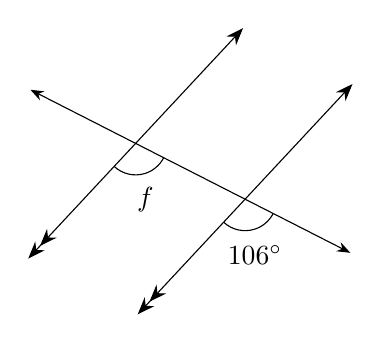
\begin{tikzpicture}[scale=1.0, baseline=(current bounding box.north)]
    \begin{scope}[rotate=153]
      % Draw the first line
      \draw[<->>, >={Stealth[scale=1.3]}, name path=P1] (0, 0) -- (1.1025494232679967, 3.8450467837532756);
      % Draw the second line with the calculated offsets
      \draw[<->>, >={Stealth[scale=1.3]}, name path=P2] (1.560449153792403, 0) -- (2.6629985770603994, 3.8450467837532756);
      % Draw the transversal through the middle of the parallel lines
      \draw[<->, >=Stealth, name path=P3] (-0.9487252883660018, 1.9225233918766378) -- (3.6117238654264012, 1.9225233918766378);
      \path [name intersections={of=P1 and P3,by=A}];
      \path [name intersections={of=P2 and P3,by=B}];
      % Draw the angle
      \coordinate (p1s) at (0, 0);
      \coordinate (p1e) at (1.1025494232679967, 3.8450467837532756);
      \coordinate (p2s) at (1.560449153792403, 0);
      \coordinate (p2e) at (2.6629985770603994, 3.8450467837532756);
      \coordinate (ts) at (-0.9487252883660018, 1.9225233918766378);
      \coordinate (te) at (3.6117238654264012, 1.9225233918766378);
      \draw pic["$f$", draw=black, -, angle eccentricity=1.8, angle radius=0.4cm] {angle=p2e--B--ts};
\draw pic["$106^\circ$", draw=black, -, angle eccentricity=1.8, angle radius=0.4cm] {angle=p1e--A--ts};

    \end{scope}
  \end{tikzpicture}
\end{equation}\vspace{1cm}
\begin{equation}
  \text{b} = \text{\dotuline{~~~~~~~}}^\circ
  \begin{tikzpicture}[scale=1.0, baseline=(current bounding box.north)]
    \begin{scope}[rotate=241]
      % Draw the first line
      \draw[<->>, >={Stealth[scale=1.3]}, name path=P1] (0, 0) -- (-3.3546822717816958, 2.1785561400601092);
      % Draw the second line with the calculated offsets
      \draw[<->>, >={Stealth[scale=1.3]}, name path=P2] (2.754117688164994, 0) -- (-0.600564583616702, 2.1785561400601092);
      % Draw the transversal through the middle of the parallel lines
      \draw[<->, >=Stealth, name path=P3] (-3.177341135890848, 1.0892780700300546) -- (2.576776552274146, 1.0892780700300546);
      \path [name intersections={of=P1 and P3,by=A}];
      \path [name intersections={of=P2 and P3,by=B}];
      % Draw the angle
      \coordinate (p1s) at (0, 0);
      \coordinate (p1e) at (-3.3546822717816958, 2.1785561400601092);
      \coordinate (p2s) at (2.754117688164994, 0);
      \coordinate (p2e) at (-0.600564583616702, 2.1785561400601092);
      \coordinate (ts) at (-3.177341135890848, 1.0892780700300546);
      \coordinate (te) at (2.576776552274146, 1.0892780700300546);
      \draw pic["$b$", draw=black, -, angle eccentricity=1.8, angle radius=0.4cm] {angle=p1e--A--ts};
\draw pic["$33^\circ$", draw=black, -, angle eccentricity=1.8, angle radius=0.4cm] {angle=p2e--B--ts};

    \end{scope}
  \end{tikzpicture}
\end{equation}\vspace{1cm}
\begin{equation}
  \text{c} = \text{\dotuline{~~~~~~~}}^\circ
  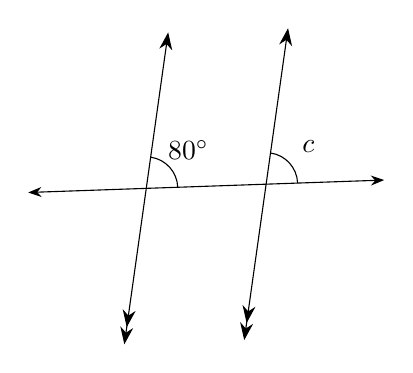
\begin{tikzpicture}[scale=1.0, baseline=(current bounding box.north)]
    \begin{scope}[rotate=182]
      % Draw the first line
      \draw[<->>, >={Stealth[scale=1.3]}, name path=P1] (0, 0) -- (0.6945927106677217, 3.939231012048832);
      % Draw the second line with the calculated offsets
      \draw[<->>, >={Stealth[scale=1.3]}, name path=P2] (1.5231399178286176, 0) -- (2.2177326284963392, 3.939231012048832);
      % Draw the transversal through the middle of the parallel lines
      \draw[<->, >=Stealth, name path=P3] (-1.152703644666139, 1.969615506024416) -- (3.370436273162478, 1.969615506024416);
      \path [name intersections={of=P1 and P3,by=A}];
      \path [name intersections={of=P2 and P3,by=B}];
      % Draw the angle
      \coordinate (p1s) at (0, 0);
      \coordinate (p1e) at (0.6945927106677217, 3.939231012048832);
      \coordinate (p2s) at (1.5231399178286176, 0);
      \coordinate (p2e) at (2.2177326284963392, 3.939231012048832);
      \coordinate (ts) at (-1.152703644666139, 1.969615506024416);
      \coordinate (te) at (3.370436273162478, 1.969615506024416);
      \draw pic["$c$", draw=black, -, angle eccentricity=1.8, angle radius=0.4cm] {angle=ts--A--p1s};
\draw pic["$80^\circ$", draw=black, -, angle eccentricity=1.8, angle radius=0.4cm] {angle=ts--B--p2s};

    \end{scope}
  \end{tikzpicture}
\end{equation}\vspace{1cm}

\end{multicols}
\end{document}
